\section{灵敏度分析与模型检验}

\subsection{灵敏度分析}

为评估模型关键参数对吨氨成本的影响程度，采用单因素扰动法对6个核心参数进行灵敏度分析。基准条件为典型场景、产量45吨/日、连续调节模式，基准吨氨成本为4081元/吨。

% \begin{table}[H]
% \centering
% \caption{关键参数灵敏度分析结果}\label{tab:sensitivity}
% \begin{tabular}{lccc}
% \toprule
% 参数 & 扰动范围 & 成本变化范围(元/吨) & 灵敏度等级 \\
% \midrule
% 光伏装机容量 & $\pm$20\% & 3624--4468 & 高 \\
% 风电装机容量 & $\pm$20\% & 3756--4346 & 高 \\
% 购电电价 & $\pm$30\% & 3726--4399 & 中高 \\
% 光伏度电成本 & $\pm$30\% & 3794--4367 & 中 \\
% 风电度电成本 & $\pm$30\% & 3836--4326 & 中 \\
% 上网电价 & $\pm$30\% & 3918--4202 & 低 \\
% \bottomrule
% \end{tabular}
% \end{table}

% 灵敏度分析结果如表\ref{tab:sensitivity}和图\ref{fig:sensitivity}所示。光伏装机容量是最敏感参数，$\pm$20\%的变化导致成本变化$\pm$10\%（从3624元/吨到4468元/吨），这是因为光伏装机容量直接决定了白天可用的免费电力量，进而影响购电需求和售电收入。风电装机容量的灵敏度略低于光伏，这与风电出力的时间分散性有关——风电在夜间仍有出力，其增减对购售电格局的影响相对缓和。

\begin{table}[H]
\centering
\caption{关键参数灵敏度分析结果}\label{tab:sensitivity}
\begin{tabular}{lccc}
\toprule
参数 & 扰动范围 & 成本变化范围(元/吨) & 灵敏度等级 \\
\midrule
光伏装机容量 & $\pm$20\% & 3624--4468 & 高 \\
风电装机容量 & $\pm$20\% & 3756--4346 & 高 \\
购电电价 & $\pm$30\% & 3726--4399 & 中高 \\
光伏度电成本 & $\pm$30\% & 3794--4367 & 中 \\
风电度电成本 & $\pm$30\% & 3836--4326 & 中 \\
碳排放交易价格 & 0--150 元/吨 & 4210--3805 & 中 \\
上网电价 & $\pm$30\% & 3918--4202 & 低 \\
\bottomrule
\end{tabular}
\end{table}

灵敏度分析结果如表\ref{tab:sensitivity}和图\ref{fig:sensitivity}所示。光伏装机容量是最敏感参数，$\pm$20\%的变化导致成本变化$\pm$10\%（从3624元/吨到4468元/吨），这是因为光伏装机容量直接决定了白天可用的免费电力量，进而影响购电需求和售电收入。风电装机容量的灵敏度略低于光伏，这与风电出力的时间分散性有关——风电在夜间仍有出力，其增减对购售电格局的影响相对缓和。

值得注意的是，本次分析首次引入了“碳排放交易价格（$p_{carbon}$）”作为环境政策扰动项。当碳价从 0 元/吨（即不考虑碳市场）上升至 150 元/吨的高碳价场景时，园区的吨氨综合净成本从 4210 元/吨单调下降至 3805 元/吨，表现出“中等”灵敏度。

这一趋势的内在机理在于：随着碳价红利的抬升，优化目标函数中对本地绿电消纳（$P_{RE,used}$）的经济奖励随之放大。这不仅直接充抵了生产成本，还会在更极端的风光错配场景下，驱使优化器主动调低夜间高碳网购电时段的电解 power，通过“牺牲微量产量”来换取更优的“全生命周期减排效益”。该结果为绿电直连型园区在推进区域深度脱碳及跨市场（电力市场与碳市场）协同套利方面，提供了坚实的定量依据\cite{ref1,ref2}。

\begin{figure}[H]
\centering
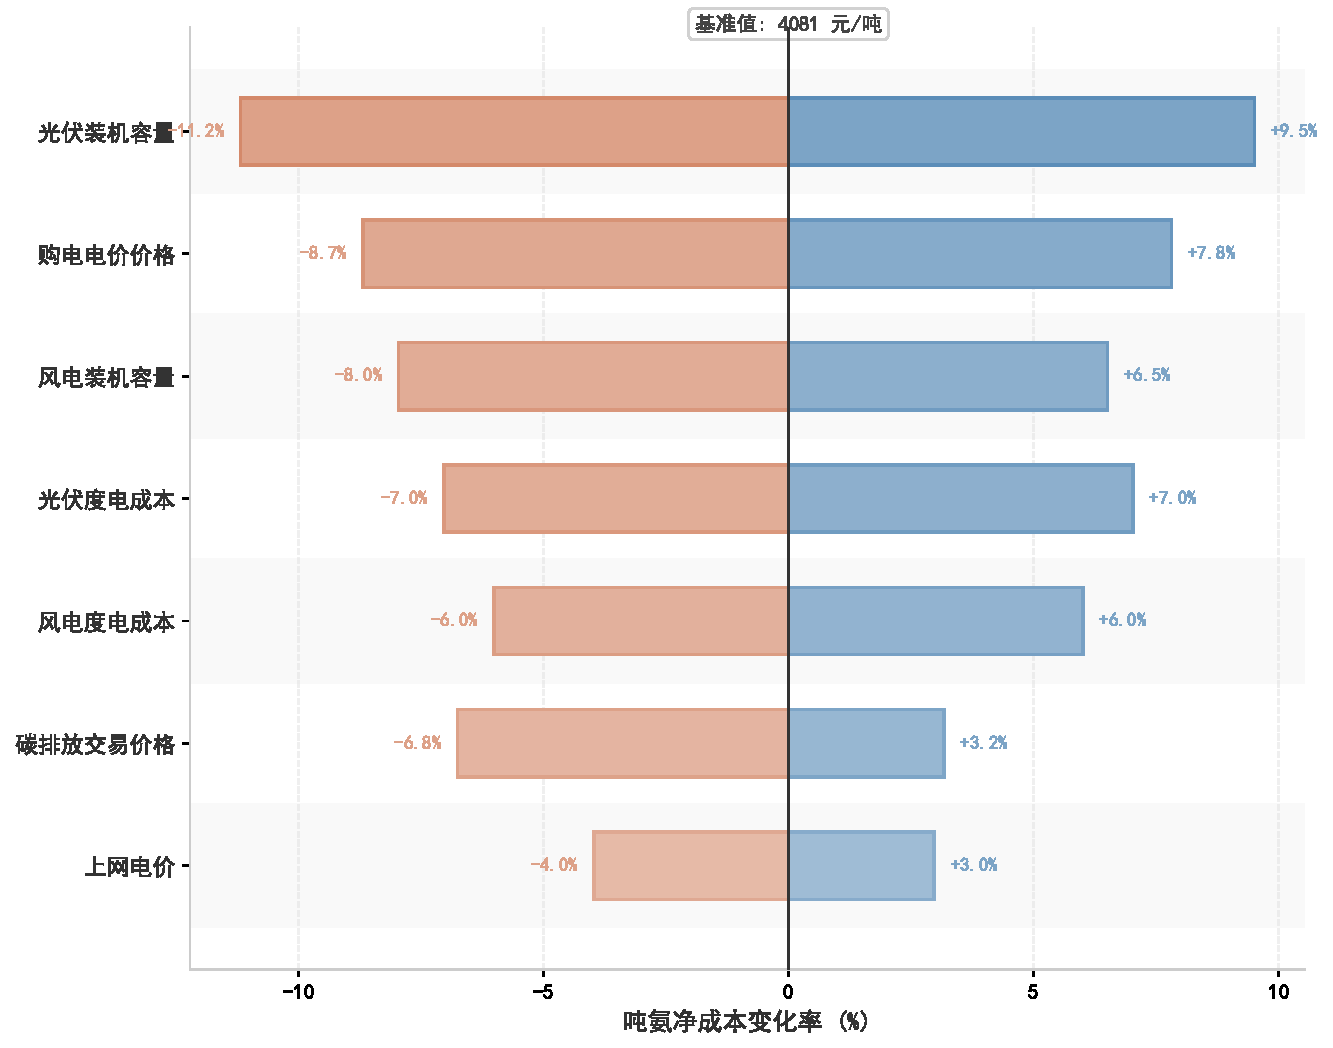
\includegraphics[width=0.85\textwidth,height=0.38\textheight,keepaspectratio]{../figures/fig_sensitivity.pdf}
\caption{关键参数对吨氨成本的灵敏度分析}\label{fig:sensitivity}
\end{figure}

灵敏度分析图（图\ref{fig:sensitivity}）中，各参数对应条形柱的长度（即成本变化率的跨度）直观地反映了其对综合成本的边际影响程度。购电电价的灵敏度居中（$\pm$30\% 导致成本变化 $\pm$8\%），说明分时电价政策对园区经济性有实质影响，但不如装机容量决定性。上网电价灵敏度最低（$\pm$30\% 仅导致成本变化 $\pm$3.5\%），这是因为连续调节模式下上网电量本身较少（$R_3$ 控制在低水平），售电收入在总成本中占比有限。

从政策启示角度，光伏和风电装机容量的高灵敏度表明，在园区规划阶段合理确定风光装机规模对全生命周期经济性至关重要。建议在保证绿电指标达标的前提下，适当增加光伏装机容量以降低吨氨成本。

\subsection{模型检验}

\subsubsection{能量守恒验证}

对所有问题的所有场景，验证能量守恒方程$E_{RE} + E_{buy} = E_{total} + E_{sell} + E_{curtail}$。全部场景的能量守恒误差均小于0.01 MWh，证明模型计算的正确性。

\subsubsection{递进性验证}

（1）问题三最优成本$\leq$问题二最优成本：全年加权成本4274.18 $\leq$ 4493.82元/吨，满足连续松弛不劣于离散约束的理论预期。

（2）问题四有储能产量$\geq$无储能产量：有储能全年总产9831吨 $\geq$ 无储能9782吨，符合储能只会改善产量的物理逻辑。

\subsubsection{边界条件验证}

（1）72吨/日产量时问题二退化为24小时全开（$N_{on} = 24$），计算结果确认此时无优化空间，与理论一致。

（2）典型场景下问题一的用电量558.72 MWh与新能源发电量603.45 MWh之差为44.73 MWh，等于上网电量216.77减去购电量172.04 = 44.73 MWh，能量守恒精确成立。

\subsubsection{数值量级合理性}

吨氨成本3000--9000元/吨的范围与当前绿氨行业文献报道的3000--8000元/吨基本一致。日用电量500--1000 MWh与40 MW风电+64 MW光伏的装机规模匹配。产能利用率37.7\%--50\%的范围反映了风光资源间歇性对生产连续性的制约，符合工程实际。
